\section{Evaluation}\label{sec:results}

%In this section, we will present our evaluation results of the \systemname.
We conducted comprehensive evaluation of \systemname~through laboratory studies involving
human subjects -- our studies were approved by the Institutional Review Board (IRB) of our
institution. In the first phase of evaluation, we collected from volunteer participants accelerometer sensor
readings with Google Glass. We analyzed these traces offline on a PC.
Our evaluations are primarily aimed at determining the accuracy of detecting
and differentiating users based on their head-movements, and understanding
the effect of important design parameters such as similarity metric, length of the music cue, training
data-set size and sampling rate. In the second phase of evaluation, We also measured the response time of our Google
Glass implementation of \systemname.

%based on profiling the execution time of each key
%functions associated with \systemname, on the Google Glass device.


\begin{figure}[t]
\centering
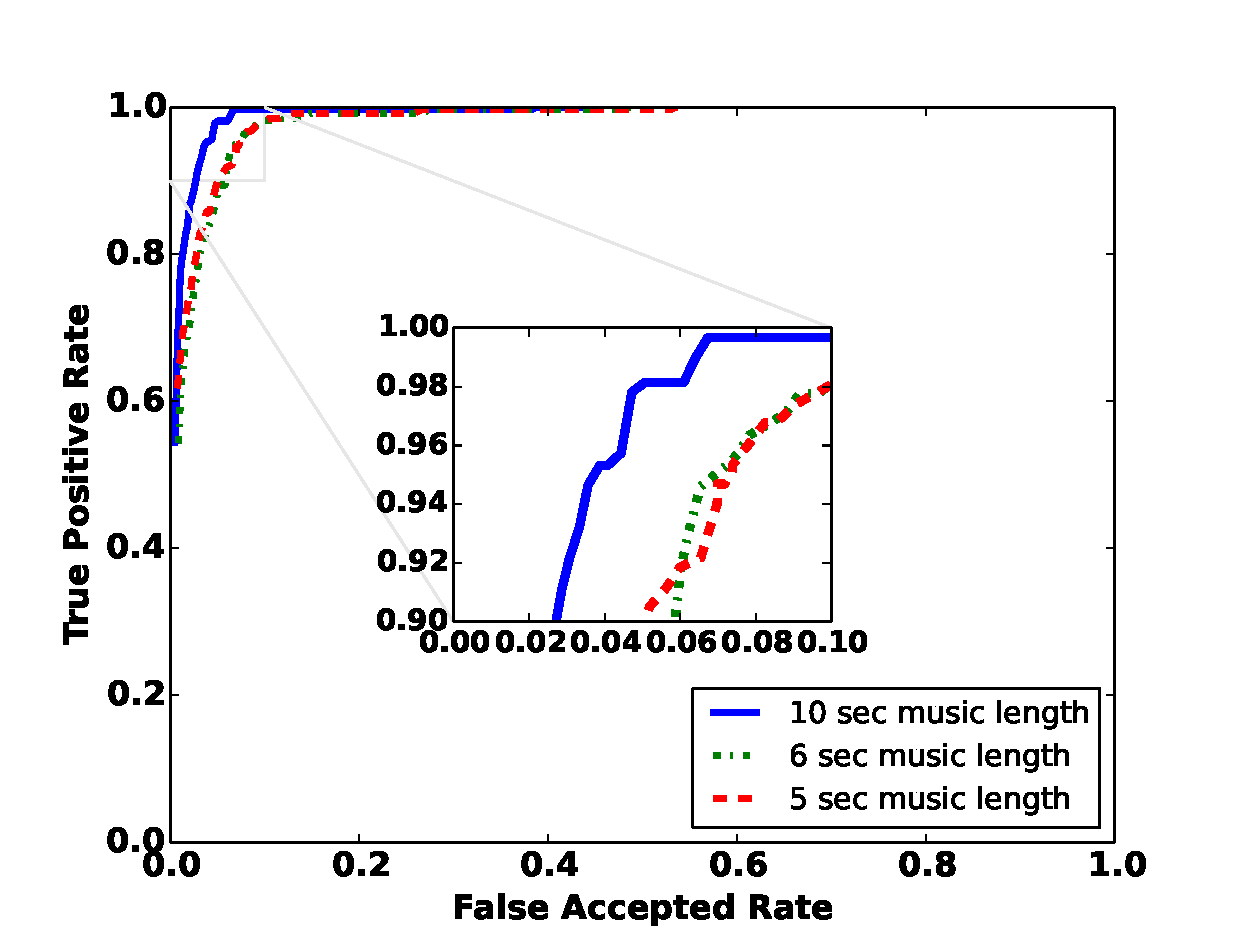
\includegraphics [width=\columnwidth]{figure/top1_roc.eps}
\caption{The impact of music cue duration on TPR and FAR in Top-1 scheme ($K = 1$). We trimmed a 10s music snapshot into music cues of 10s, 6s and 5s correspondingly. In this set of results, we varied $n$ ***YZ: what is n? What are the values n? Please specify ***}
%The variable here is $n$. Each (TPR, FAR) data point in the curve corresponds to a different value of $n$}
\label{fig:roc-top1}
\end{figure}

\begin{figure}[t]
\centering
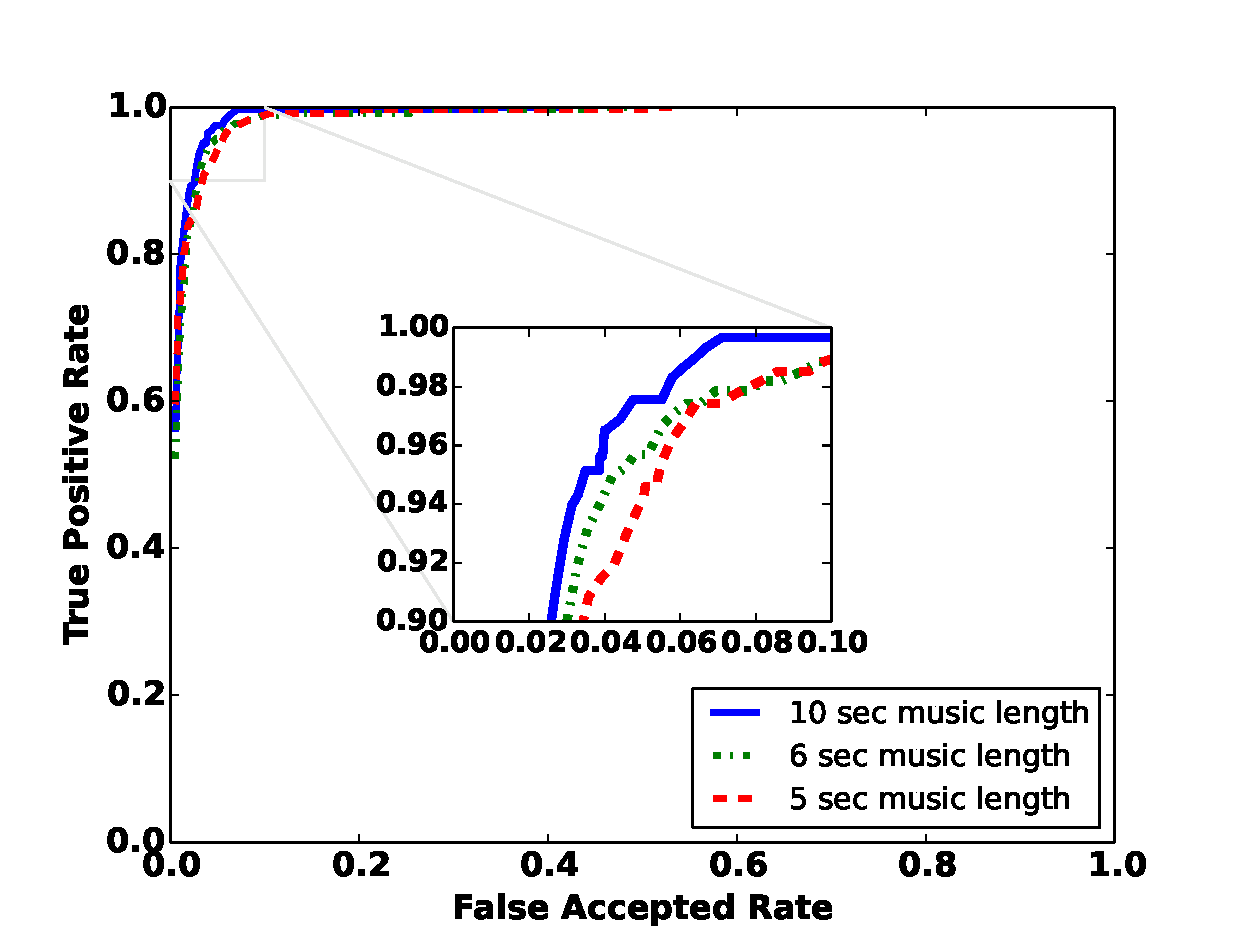
\includegraphics [width=\columnwidth]{figure/top3_roc.eps}
\caption{Evaluation of impact of music cue duration on TPR and FAR in Top-3
voting scheme ($K = 3$). A 10 sec music snapshot is trimmed into music cues of
10 sec, 6 sec and 5 sec correspondingly.The variable here is $n$. Each (TPR, FAR) data point in the curve corresponds to a different value of $n$}
\label{fig:roc-top3}
\end{figure}

\begin{figure}[t]
\centering
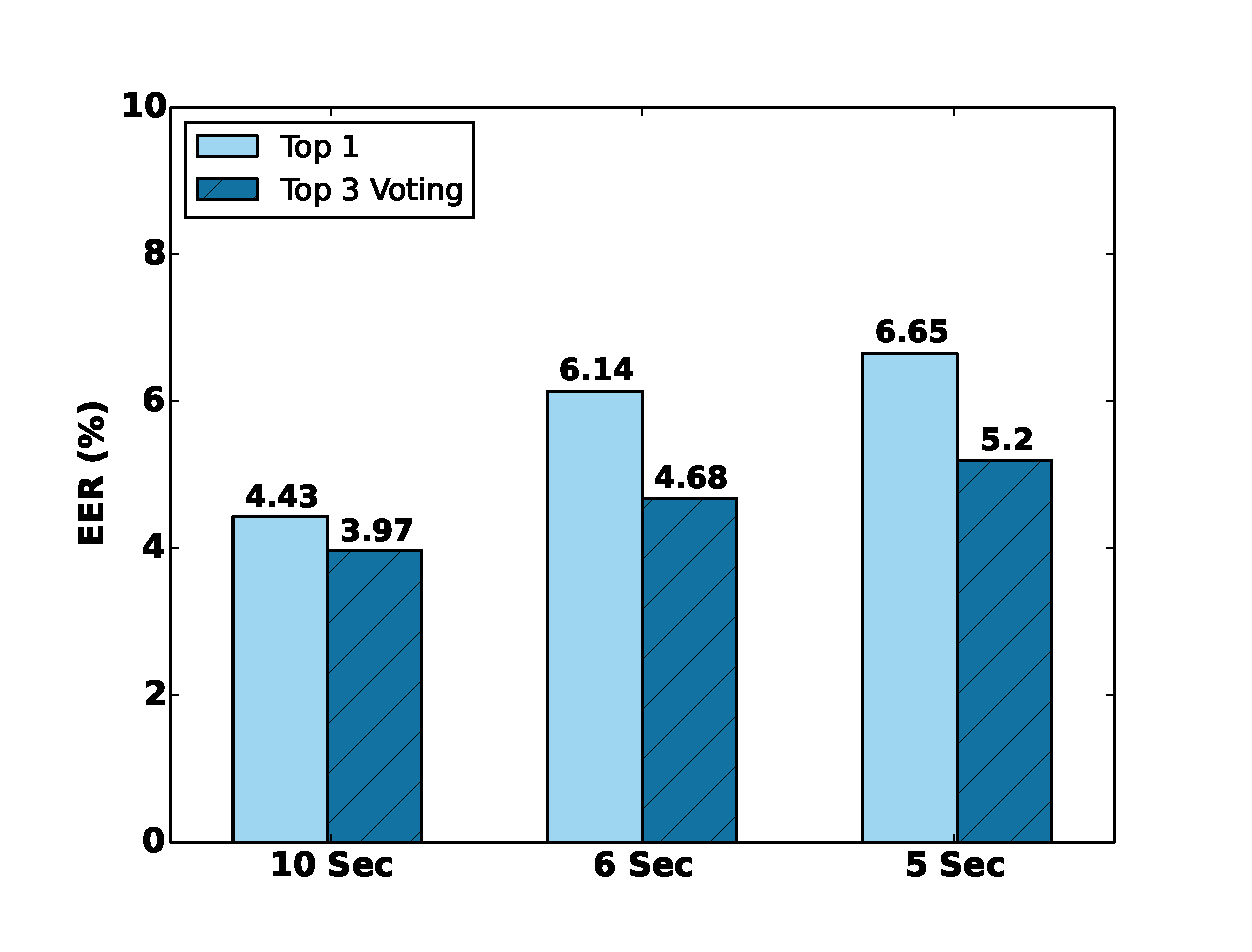
\includegraphics [width=\columnwidth]{figure/exp2_vary_length.eps}
\caption{Comparison of EER for different music lengths (10 sec, 6 sec and 5
sec) with a fixed n value of 2.7}
\label{fig:eer-length}
\end{figure}

\begin{figure}
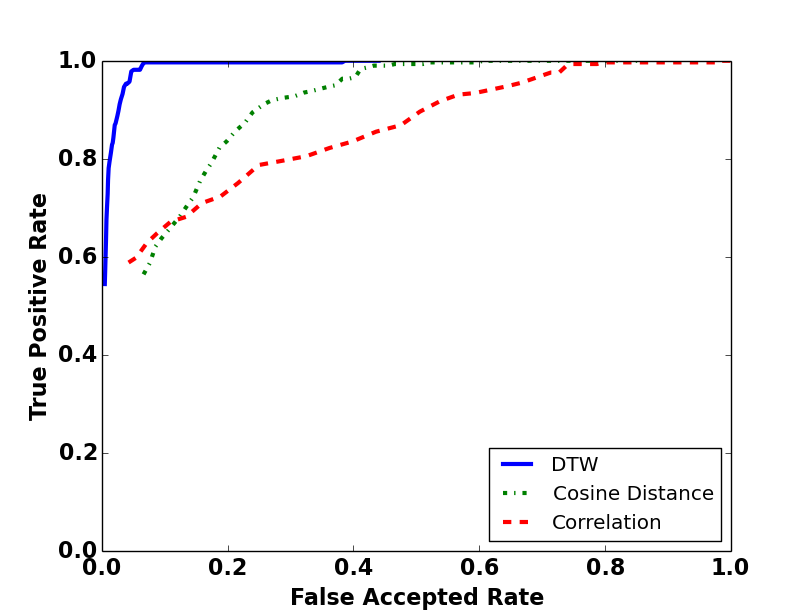
\includegraphics[width=\columnwidth]{figure/roc_dtw_cos_cor.png}
\caption{\label{fig:roc_dtw_cos_cor} Evaluation of impact of different distance metric (DTW, cosine distance, and Correlation). Although DTW is relatively computing-intensive, ROC curve indicates  that DTW provides a large enhancement over the other two metrics. }
\end{figure}

\begin{figure}
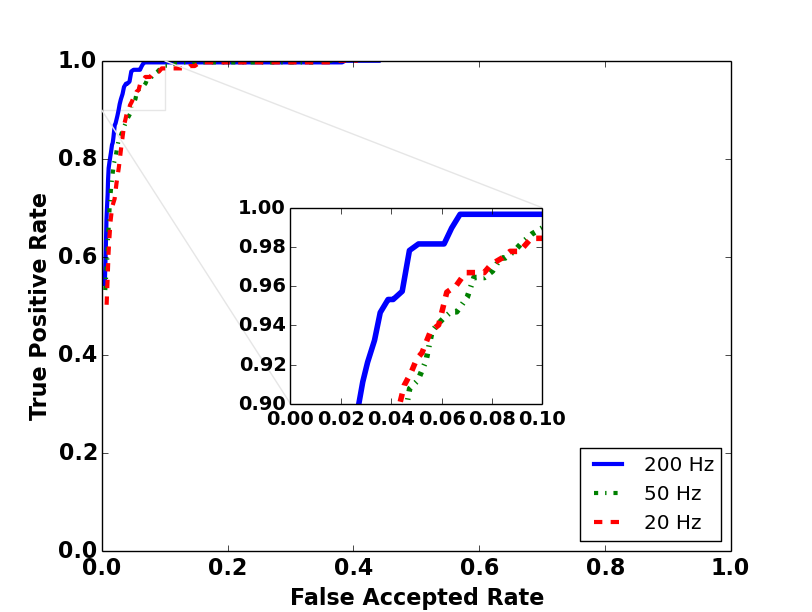
\includegraphics[width=\columnwidth]{figure/roc_dtw_diff_freq.png}
\caption{\label{fig:roc_dtw_diff_freq} Evaluation of impact of different sampling rate shows that the highest sampling rate 200 Hz gives the best resutlt. However, the sampling rate determines computational effort for the smart device, which could be significant in terms of response time.}
\end{figure}


\subsection{Authentication Accuracy of \systemname}

\subsubsection{Participants}
We had a total of 30 volunteer participants for this experiment, including a total of 19 males and 11 females.
The average age of the participants was 29.7 years with a standard deviation
of 9.81 years. The youngest participant was 23 years old while the eldest was
54 years old.

\subsubsection{Procedure}
Our first experiment setup aimed at emulating the typical usage scenario
of \systemname~for authentication, where a user conducts head-movements in
response to a music cue played on the Google Glass device during a login
attempt.
%One of the participants executing the experiment trial wearing the
%Google Glass. %Figure~\ref{fig:setup} shows our experiment setup.
In this experiment, all participants were asked to wear a Google Glass
device. Participants who originally wore spectacles were asked to remove their
spectacles before conducting the experiment.
The trials were conducted in an academic environment and overseen by one of
our team members.
The Google Glass ran our data-collection app that played a piece of
music (music cue) for a specific duration, and recorded the accelerometer
sensor readings. We conducted these trials for three duration values: 5s,
6s and 10s. %As we will show further, the accuracy of the system can
%significantly improve with the duration of the music cue; longer the duration
%better is the accuracy.
The sensor readings were recorded into a text file that was stored
in the Glass's memory and later transported to a PC for offline processing
through a Python script. The experiment was conducted in a well-lit indoor
academic laboratory environment.

During the course of a data collection session, the participants were allowed to take a
break or withdraw from data collection if they felt uncomfortable at any
point; for example, feeling
dizzy after head-movement for a period of time, not being able to see clearly
if near-sighted, etcetera. The conductor also allowed the user to take a break
of about one minute after each trial.
Each trial lasted for the duration of the music cue played on the Glass, and
a total of 40 such trials were conducted for each of the 30 subjects.
The entire data collection effort lasted over a duration of 60 days, of which 15
subjects conducted their trials in a single sitting over a period of two
hours, while the rest of the trails were spread over 3 days on an average per
subject.
%while, half of the trials of the rest 10 subjects were spread over 2 days.
The experiment yielded three sets of data traces that each correspond to
the three music cue durations we selected.

\subsubsection{Results}
We evaluate the accuracy of \systemname~using metrics that are commonly used
in evaluating authentication systems, namely,
the false acceptance rate FAR (percentage of false test samples that are
mistakenly accepted), false rejection rate FRR (percentage of true test
samples that are mistakenly rejected), and true positive rate
TPR (percentage of true test samples that are correctly accepted).
A strict threshold in the classifier can lead to high FRR, while
overly relaxing the same can lead to a high FAR. Hence, we also consider
the equal error rate EER (percentage of errors when $FAR = FRR$), that
considers both FAR and FRR.
%and balanced accuracy BAC, where BAC = 1 - (FAR+FRR)/2.
%We present the accuracy results through the receiver operating
%characteristics (ROC) curves, TPR versus FAR, as shown in Figures~\ref{}
%and~\ref{}.
Figures~\ref{fig:roc-top1}, \ref{fig:roc-top3} and \ref{fig:eer-length} report
the accuracy
of \systemname~through the metrics stated above.
%Figures~\ref{fig:roc-curves} (a)-(c) report the accuracy of
%\systemname~through the metrics stated above.

In general, we observe that even with a 5s music cue, \systemname~can achieve a TPR of ***\% at FAR of ***\% and EER of ***\% (when we have $K$=***, *** out of 40 trials from each user being used for training with  thresholding parameter value $n = 2.7$ with DTW). If users do not mind a cue duration of 10s, the TPR can be as high as 95.1\% at FAR of 3.5\% and EER of 3.97\% (when we have $K = 3$, and 30 (out of 40) trials from each user being used for training with a thresholding parameter value $n = 2.7$ with DTW).
Next we discuss in more detail how the authentication accuracy results are impacted by various design parameters.

\paragraph{Impact of similarity algorithm}
In previous preliminary study, we find that DTW, Cosine Distance, and Correlation are giving promising results for the response time sequence, hence we will evaluate these three algorithms in our end-to-end system. Also due to DTW is relatively more computing-intensive than the other two algorithm, we would like to see whether DTW  is worth of computing resource. In this experiment, we vary thresholding parameter value $n$ and fix the other parameters: 10 sec duration, $K = 1$, and  training data $size = 30$. We can observe from the ROC
(receiver operating characteristic) curves in Figure~\ref{fig:roc_dtw_cos_cor} that DTW gives the best result among three algorithms, since its curve is the closest to the upper left corner. Our system preserves all characteristics of the data, which includes the response time to the music beat and the 3-axis accelerometer data. In terms of matching the waveform of two signal, DTW can achieve significant enhancement than the other two algorithms~\cite{DTW}.

\paragraph{Impact of music cue duration and $K$ value}

The classification algorithm in \systemname~generates the classification result (YES or NO) by voting among the individual results each generated by the top-K samples in the truing set. We can observe from the ROC curves in Figure~\ref{fig:roc-top1} and \ref{fig:roc-top3} that
for both, $K=1$ and $K=3$, the TPR is close to 95\% while the FAR is slightly
above 3\% for the 10 sec music duration. For $K = 1$ the FAR increases to
about 7\% for the 5 sec and 6 sec cases, however, for $K = 3$ the FAR
decreases to about 3\% and 4\%, respectively.
We observe a similar trend with the EER as shown in
Figure\ref{fig:eer-length}, where improvements of 0.5 - 1 \%
can be achieved by choosing $K = 3$ over $K = 1$.
This indicates that the accuracy in \systemname~can improve with a larger
value of $K$. However, the improvement in accuracy through redundancy in the
training set trades off with the increased execution time as the
matching requires at least $K - 1$  extra DTW computations as opposed to only
1 for a top-1 scheme. As we will show ahead, DTW computations incur heavy CPU
budget on the wearable device.
%We measure the DTW computation on Google Glass to be the most
%computationally expensive operation of all the software modules in
%\systemname.
%\paragraph{Impact of music cue duration}

In general, we observe from the results that the FAR can
be decreased by increasing the music cue duration.
We can observe (from Figures~\ref{fig:roc-top1}, \ref{fig:roc-top3} and
\ref{fig:eer-length}) that the improvement is less significant when the music
cue duration is increased from 5 sec to 6 sec, however, the improvement is
more
significant when the music cue duration is increased to 10 sec.
In \systemname~the data collection phase for the authentication system
(sampling accelerometer sensor readings) is executed in parallel with the
music cue. The data processing phase involving the filtering, classification
and matching is executed only at the end of the music cue and in the same
order.
%Hence, execution time of the app will be independent of this duration.
We note that, the data input duration of 5-10 sec for authentication
may seem long, but in reality, such data input durations are on par with those
of password based systems~\cite{von2013patterns}.
%We also note that, since the authentication process is initiated only at the
%end of the music cue, execution time of the app will be independent
%of this duration.

\begin{figure}[t]
\centering
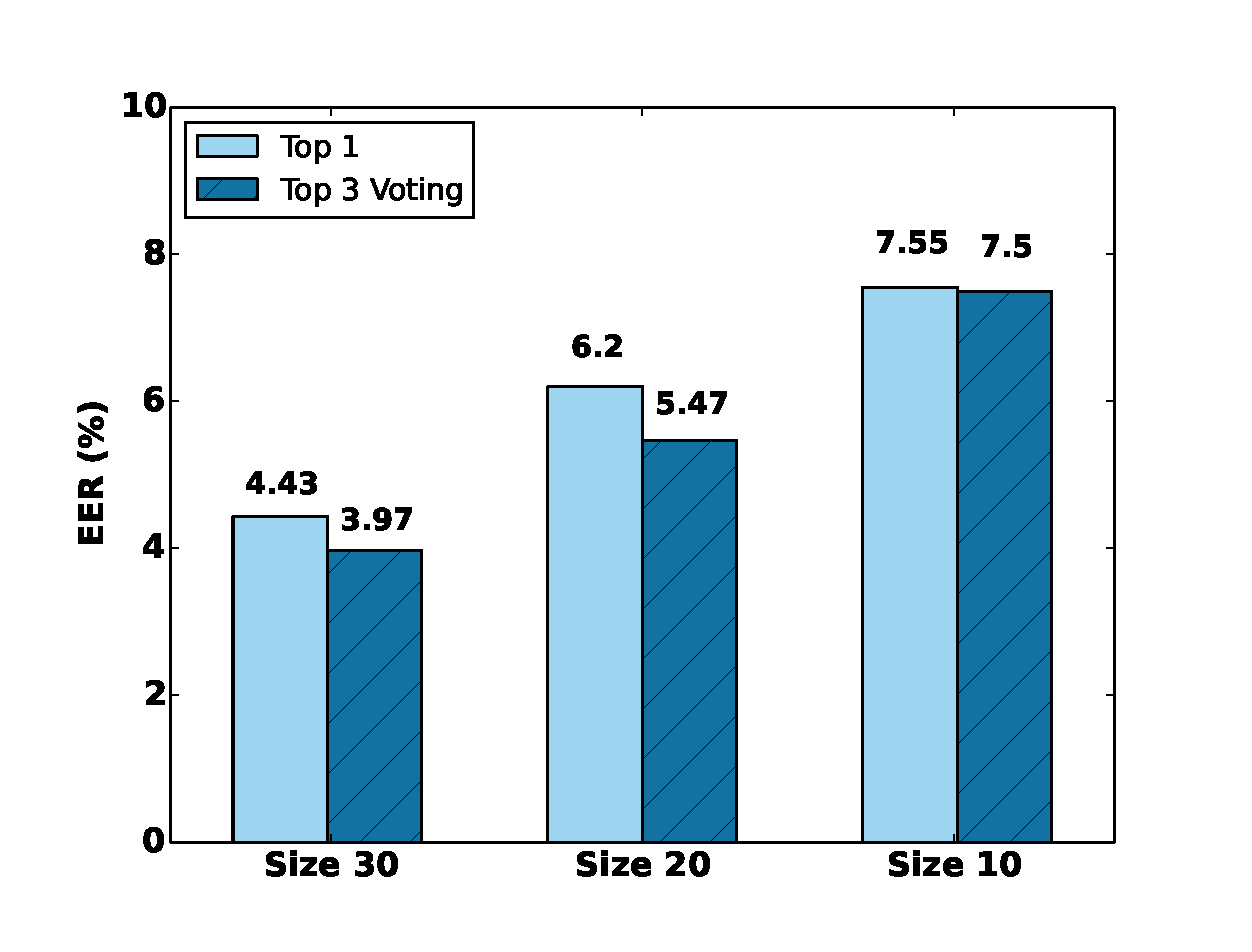
\includegraphics [width=\columnwidth]{figure/exp2_vary_size.eps}
\caption{Comparison of EER for different training sample sizes (30, 20 and 10)
with fixed n value of 2.7}
\label{fig:eer-size}
\end{figure}


\paragraph{Impact of Training Set Size}
%The accuracy of detecting and matching the head-movements to the user depend
%upon the music cue duration, value of $K$, and number of samples used for
%training.
Recalling from \systemname section~\ref{sec:design}, the input to the training phase
is a set of temporal signals (samples with duration equal to the music cue
duration), each corresponding to one trial of the head-movements from the
user. Our evaluations so far considered a training set size of 30 samples.
In Figure~\ref{fig:eer-size}, we report the EER in \systemname~for three
different training data set sizes; 10,20 and 30 samples.
We can observe from Figure~\ref{fig:eer-size} that the EER holds an inverse
relationship with the training set size. A larger training set minimizes the
variance in mean and standard deviation computations, as the errors in their
inconsistency are reduced by averaging the mean and standard deviation
estimates over a larger set of data.
On the other hand, a larger training set also implies a longer execution time
of the training phase.
However, in our system design, we posit that the training phase can be
conducted
offline on a more compute efficient device (smartphone, PC or server) and that
the wearable device can pre-fetch the trained data (for example, an XML file),
prior-to or during data collection phase, through a wireless link.
\paragraph{Impact of Sampling Rate}
Due to DTW is resource-consuming, one direct way to reduce the workload of our algorithm is to decrease the sampling rate of the accelarometer and remain the sampling time. Based on Nyquist–Shannon sampling theorem, since the high cut of our filter is 10 Hz, the minimum sampling rate should be 20 Hz. Also, the highest sampling rate and the default sampling rate of our platform are 200 Hz and 50 Hz accordingly. Thus, we choose these three value to evaluate the impact of sampling rate.  In Figure~\ref{fig:roc_dtw_diff_freq}, we observe that 200 Hz provides the best performance among three value, while 50 Hz and 20 Hz are giving closed results. The EER of 20 Hz is **, comparing with  ** of that of 200 Hz. Since the decrement of EER is insignificant and we can achieve 10 times speedup in DTW computing,  20 Hz will be a ideal value of system implementation.
\begin{figure}
\centering
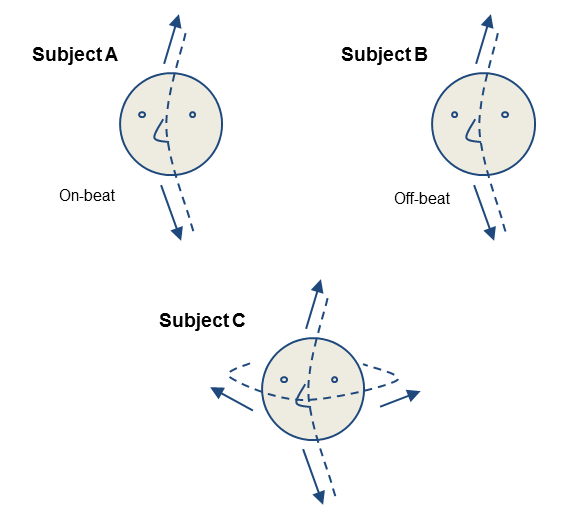
\includegraphics[width = \columnwidth]{figure/imitation_subject_movement.png}
\caption{\label{fig:imitation_movement} Pictorial description of how the mimicked subjects move.}
\end{figure}


\subsection{Is it hard to imitate?}
\subsubsection{Participants}
We had total of 38 volunteer participants. The participants list included a total of 32 males and 6 females.
The average age of the participants was 25.6 years with a standard deviation
of 6.6 years. The youngest participant was 22 years old while the eldest was
at 49 years.
\subsubsection{Procedure}
Our second experiment aimed at an practical imitation attack field test scenario. In this experiment, three subjects were taken video while they were performing their successful login movement. Note that the music cue is usually played via a bone conduction speaker or a earplug, hence a camcorder is difficult to capture the music sound if the environment is noisy or the microphone is not sensitive enough. In this case, the imitators will be impossible to synchronize the music with the video. To eliminate this concern, we set the volume of the speaker to maximum and took the video in a quiet laboratory environment.

The participants were divided into three group, and each group was asked to imitated only one of the three users above. During the test, the participants could watch the video for as many time as their willing at anytime between two trials. A feedback from our system would be provided after each trail so that the participants could decide whether they needed to adjust their movement or not. After total number of trials reached 30 for each participant, the experiment would stop regardless the participant succeed or not. The investigator was not only recording the total number of successes, but also the number of trail before the first successful login. This experiment was conducted in quite space on campus. We will now discuss our evaluation results for both experiments in detail.

\subsubsection{Results}
Although it is difficult to quantitatively to describe the complexity of the movement in 5-Dimension space(3-axis accelarometer, time space,  and response to the music beat), there are some distinguish characteristics of these three subjects, hence they are chosen to become our imitated subjects. As shown in Figure~\ref{fig:imitation_movement} $Subject A$ performed a simple nodding movement by naturally following the music flow. $Subject B$ also performed a simple nodding, but his movement was always off-beat with the music. $Subject C$ performed a movement combined with nodding and shaking, and he only nodded/shake at certain beats instead of every beat, which makes his movement is relatively difficult to learn. Table~\ref{tab:imitation} shows the overall result of this experiment. The overall FAR is 7.54 \%, while the individual FARs are 17.67\%, 9.82\% and 3.27\% accordingly.  Since $Subject A$ perform the simplest movement among these three subjects, 6 out 10 subjects could succeed at least once during their 30 trials, while for $Subject B$ and $Subject C$ this number is 3 of 15 and 3 of 10.

\begin{table}[]
\centering
\label{my-label}
\begin{tabular}{lcccc}
\hline
                            & \multicolumn{1}{l}{Total Imitator} & \begin{tabular}[c]{@{}c@{}}Successful Imitator \\ Number\end{tabular} & \begin{tabular}[c]{@{}c@{}}Average Number of \\ Trial before \\ First Successful Login\end{tabular} & \multicolumn{1}{l}{FAR (\%)} \\ \hline
Subject A                   & 12                                 & 7                                                                     & 10.33                                                                                               & 15.83                        \\ \hline
Subject B                   & 13                                 & 3                                                                     & 14.33                                                                                               & 2.77                         \\ \hline
Subject C                   & 12                                 & 3                                                                     & 17.67                                                                                               & 2.72                          \\ \hline
\multicolumn{1}{c}{Overall} & 38                                 & 13                                                                    & 13.17                                                                                                    & 6.94                         \\ \hline
\end{tabular}
\caption{\label{tab:imitation}Imitation attack experiment result. Successful Imitator Number represents the number of the imitators that succeed at least once. Average Number of Trail before first login indicates the average times of trail a successful imitator takes before the first login.}
\end{table}



\subsection{Headbanger Google Glass App Implementation}

\begin{figure}[t]
\centering
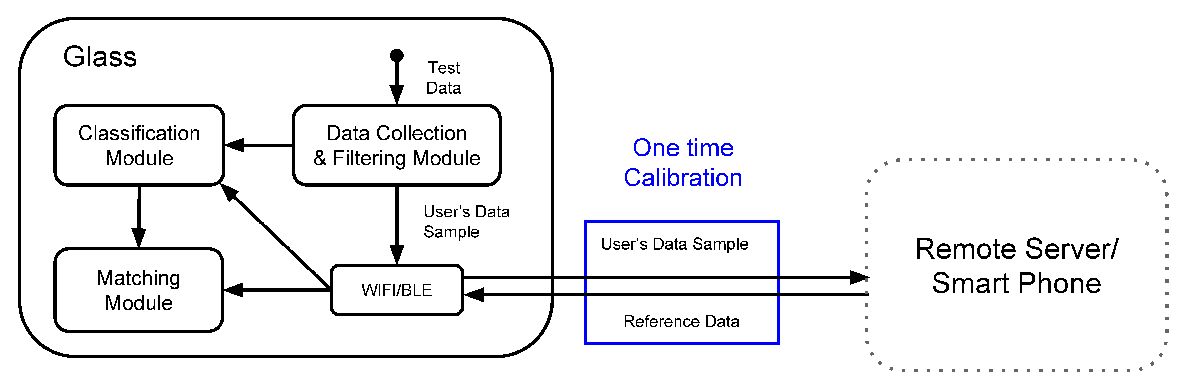
\includegraphics [width=\columnwidth]{figure/software_arch.eps}
\caption{Software modules of \systemname~implementation}
\vspace{25 pt}
\label{fig:glass-softwarearch}
\end{figure}

We implemented \systemname~on Google glass, positioning it as an
authentication application (app).
Figure~\ref{fig:glass-softwarearch} shows the main software modules in the
app. Upon initiation by the user, the app plays a music cue for a stipulated
duration. The user conducts head-movements in synchrony with the music cue
while the app records the accelerometer sensor in parallel. At the end of the
music cue duration the app executes the data processing phase where the
sensor readings are input to the \systemname's software modules for
processing. The processing stage includes the filtering of the accelerometer
sensor values, classification and feature extraction using DTW, and threshold
based matching of the generated features with those from training set.
%\systemname extracts the head-movement features through
%the thresholding process discussed in section~\ref{sec:design}, and compare
%with the feature templates generated from the training phase.
Upon completion of data processing, the app responds with a YES or NO textual
output on the Google Glass screen, depending on match score.

In our current implementation, the training phase is conducted offline, prior
to live-testing off the application.
The training phase involves collecting 30 samples (variable) of the
head-movement accelerometer readings, generating the features, and saving them
into a local server (running on PC) as an XML file, with appropriate indexing.
Upon app initiation on Glass, the trained features are pre-fetched from
the server through a wireless connection. This ensures that the training set
is readily available during the authentication process, thus eliminating the
additional processing time required for the training phase.
Conducting online training, particularly that involves DTW computations, is
very compute intensive on a resource constrained devices such as Glass.
One possible solution would be for the Glass to offload the
training phase computation to a local server machine.
%We reserve such considerations for future implementations.

%Among all the software modules, the ``training set construction model'' is
%the most computing-intensive, and as a result, we executed the model on the
%bluetooth-paired smartphone. The rest of the modules are implemented and
%executed on the glass.
%In our on-glass app, the classification module runs the
%thresholding-based classification.
\subsubsection{Response time}

\begin{table}
\centering
\begin{tabular}{|ccclc|}
\hline
\multicolumn{1}{|c|}{\multirow{2}{*}{\begin{tabular}[c]{@{}c@{}}music  cue \\
duration (s)\end{tabular}}} &
\multicolumn{1}{c|}{\multirow{2}{*}{\begin{tabular}[c]{@{}c@{}} response\\
time (s)\end{tabular}}} & \multicolumn{3}{c|}{time breakdown (\%)}
\\ \cline{3-5}
\multicolumn{1}{|c|}{}
                             &
\multicolumn{1}{c|}{}
                              &
 Filtering & \multicolumn{1}{c}{DTW} & Thresholding   \\
 \hline\hline
10
                             &
1.93
                              &
 0.50      & 99.50                   & \textless0.01  \\
6
                             &
1.15
                              &
 0.64      & 99.36                   & \textless0.01  \\
5
                             &
0.88
                              &
 0.81      & 99.19                   & \textless0.01 \\ \hline
\end{tabular}
\caption{\label{tab:glass} Measured response time of \systemname~app implementation on Google
Glass with different music cue durations and for $K = 1$. The response time
reported here is an average over 20 trials.}

\end{table}

In Table~\ref{tab:glass} we report the measured average response-time
of the \systemname implementation on Google Glass app for music cue durations
of 5,6 and 10 seconds. We conducted the benchmark execution-time profiling of
\systemname~on Glass in a controlled indoor laboratory setting with no
mobility. We define response time as the time elapsed between music cue
completion to
the display of authentication response (YES/NO text) on the Glass screen.
Our measurements indicate that the response time is within 5 seconds for a 10
second data input, and is almost halved for a 5 second data input.
We feel that a response time of 2-5 sec for a local authentication solution in
Google Glass is comparable to that of prior-art that comes close to our
solution~\cite{von2013patterns,egelman2014you}.
It is also important to note that authentication solutions that execute
locally on head-worn wearable devices, especially on a heavily resource
constrained device like Glass, are still not mature. However, the hope is that
such solutions will possibly catch up to speed in the near future and that our
approach is advancing one step in that direction.
In Table~\ref{tab:glass} we also report the execution time of the key
processes in \systemname; filtering, DTW computation ($K = 1$ requires 1 DTW
computation), thresholding based similarity matching.
We can observe from Table~\ref{tab:glass} that the DTW computation
dramatically compute intensive than the other processes.

It is important to note that our current implementation uses a faster
version of the DTW algorithm called Fast DTW~\cite{salvador2007toward},
providing about 2x speed-up in DTW computation.
We believe that the response time can be reduced
further through strategic methods such as, further optimizations in the Fast
DTW algorithm or pipelining the app execution along with data collection.
A specific strategy for reducing response time for rejected attempts can be
that, after a short duration, before the entire music cue is played, if it is
found that a user's movement does not match the signature of the claimed user
with a sufficient pre-determined confidence level, then the on-site
classification may be terminated instead of waiting for the entire duration to
yield the rejection.
Another example, may include cyber-foraging strategies to offload heavy
computation tasks, such as online training and classification, to the user's
Bluetooth paired smartphone or a nearby cloudlet~\cite{ha2014towards}.

